\section{Optimal Policy Solver with Arbitrary Per-Layer Costs}
It is important to have a firm grasp of Algorithm \ref{alg:2-policy-solver} before reading this section.

Let us restate the exact problem it is solving, which is for a sequence of uniform layers:

\textit{Find the optimal cost }\(C(t,\,m)\)\textit{ for performing backpropagation on a sequence of length }\(t\)\textit{ within }\(m\)\textit{ memory slots, using checkpointing.}

How do we generalise this to take into account precise per-layer compute and memory costs?
In this section, I will explain this by deriving the shortcomings of the original policy solver when tasked with handling per-layer costs, and then showing how to overcome them.

%%%%%%%%%%%%%%%%%%%%%%%%%%%%%%%%%%%%%%%%%%%%%%%%%%%%%%%%%%%%%%%%%%%%%%%%%%%%%%%%
\subsection{Introducing Per-Layer Costs}
Let \(\alpha : \{f,\, b\}\times[0,\, N+1] \rightarrow \R^+\) and \(\beta : \{f,\, b\}\times[0,\, N+1] \rightarrow \Z^+\) be the per-layer forward and backward compute costs and memory costs, respectively, denoted \(\alpha^f_i\) for the computational cost of the \(i^\mathrm{th}\) forward, for example.

We can no longer talk about arbitrary sequences of length \(t\), as each individual subsequence of length \(t\) will have different costs as defined by \(\alpha\) and \(\beta\).
Thus the cost function now becomes \(C(i,\, j,\, m;\, \alpha,\, \beta)\), and similarly the policy \(D(i,\, j,\, m;\, \alpha,\, \beta)\).
The parameters \(\alpha\) and \(\beta\) will be omitted for brevity when it is clear from the context what they are.

The exact definition of \(C(i,\, j,\, m;\, \alpha,\, \beta)\) becomes:

\textit{Given }\(f_i\)\textit{ and }\(b_j\)\textit{, the optimal computational cost according to }\(\alpha\)\textit{ and }\(\beta\)\textit{ to perform backpropagation on the segment, that is to compute }\(b_i\)\textit{, within }\(m\)\textit{ remaining memory, using checkpointing.}

To recap what these tensors are, consider the simplified computational graph for backpropagation not including the weights given in Figure \ref{fig:3-comp-graph}, as derived in Section \ref{sec:2-4-2-peak-mem-training}.

\begin{figure}[h]
    \centering
    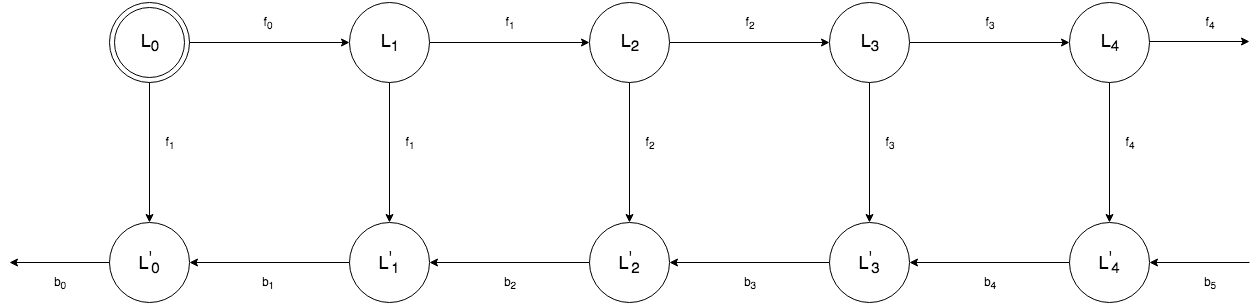
\includegraphics[width=0.95\linewidth]{simplified_comp_graph.png}
    \caption{Computational graph for backpropagation on a sequence, not showing the parameters.}
    \label{fig:3-comp-graph}
\end{figure}

Layer \(i\)'s forward operator takes input \(f_{i-1}\) and produces \(f_{i}\).
Its backward takes \(f_i\) and \(b_{i+1}\) and produces \(b_i\).
The network inputs are \(f_0\) and the targets are \(b_{N+1}\), for an \(N\) layer network.

Now that we have this all defined, we can think about how it affects the solver algorithm.

%%%%%%%%%%%%%%%%%%%%%%%%%%%%%%%%%%%%%%%%%%%%%%%%%%%%%%%%%%%%%%%%%%%%%%%%%%%%%%%%
\subsection{Traversing the Subproblems Bottom-Up}
Iterating over the search space bottom-up no longer means iterating over increasing sequence length \(t\), but over all possible subsequences in `subproblem order' - when we reach the subsequence \((i,\, j)\), we should have already solved all \textit{its} subproblems.
We can break this down recursively by saying that for any \(i < k < j\), we have already encountered all subsequences of \((i,\, k)\) and \((k,\, j)\).
Note, given my formulation of the computational graph, only subsequences where \(i < j\) are defined, so \((i,\, i)\) is not a valid subsequence.

\begin{figure}[h]
    \centering
    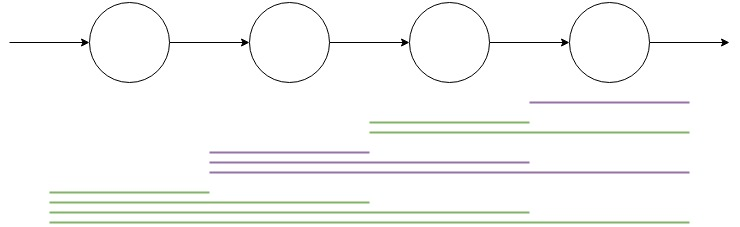
\includegraphics[width=0.8\linewidth]{subproblem-order-traversal.jpg}
    \caption{Visualisation of traversing all subsequences in `subproblem order'. The vertical bars represent a subproblem \((i,\, j)\). Traversal order goes from top to bottom. Notice that, whenever an \((i,\, j)\) is encountered, all of its subproblems have already been done.}
    \label{fig:3-subproblem-order-traversal}
\end{figure}

The way in which I traverse the subsequences is visualised in Figure \ref{fig:3-subproblem-order-traversal}.
For some sequence \((s, e)\), we will traverse all subsequences using iterators \(i\) and \(j\).
We start at the end, that is \(i = e-1\) and \(j=e\).
We cannot move \(j\) further right.
We have now solved for all subsequences that start with \(i = e-1\).
We move \(i\) left one to \(e-2\) and initialise \(j\) to the first one to the right of \(i\), \(e-1\).
Now, as we move \(j\) further right, we have already done (memoised) all the subproblems \((i^\prime,\, j)\), where \(i^\prime > i\).
In this case, that means we have done all subsequences starting with \(i=e-1\), which is true.
This means that, whenever we are considering a problem \((i,\, j)\), we have already solved all subproblems of \((i,\, i^\prime)\) and \((i^\prime,\, j)\), so never need to go `down' more than one level, but can use the memoised results.
Once we have moved \(j\) all the way right, we have now done all subproblems for \(i \geq e-2\).
Again, we move \(i\) left one to \(e-3\) and initialise \(j\) to \(e-2\).
Once we have solved this case, we move \(j\) right, knowing that we have already solved all \((i,\, i^\prime)\) and \((i^\prime,\, j)\), for all \(i' \geq i\).
We keep traversing like this until eventually we have moved \(i\) left to \(i\), and then \(j\) right to \(e\).

%%%%%%%%%%%%%%%%%%%%%%%%%%%%%%%%%%%%%%%%%%%%%%%%%%%%%%%%%%%%%%%%%%%%%%%%%%%%%%%%
\subsection{Redefining \texorpdfstring{\(Q(\cdot)\)}{\textit{Q()}} with Per-Layer Costs}
To recap, so far we have introduced per-layer costs, redefined the problem to be on all possible subsequences, and seen how to set up the solver to traverse the subsequences bottom-up.
Next, we give the new definition of the cost-action function that takes into account the per-layer costs:
\begin{equation} \label{eqn:3-Q-1}
    Q(i,\, j,\, k,\, m) \;=\; \sum_{l \;=\; i\,+\,1}^k \alpha^f_l \;+\; C(k,\, j,\, m\,-\,\beta^f_k) \;+\; C(i,\, k,\, m)
\end{equation}
This is the same as before, except we now incur the \textit{precise} costs of executing the forwards to \(f_k\), and recurse on the right with the \textit{precise} reduction in memory from checkpointing \(f_k\).
Note \(f_i\) is given by the definition of the problem so we start the sum of the forwards at \(f_{i+1}\).

%%%%%%%%%%%%%%%%%%%%%%%%%%%%%%%%%%%%%%%%%%%%%%%%%%%%%%%%%%%%%%%%%%%%%%%%%%%%%%%%
\subsection{Handling the Continuous Memory State by Tracking the Peak Memory Cost of Subproblems \texorpdfstring{\(B(\cdot)\)}{\textit{B()}}}
However, all is not so simple.
The fact that we are now being precise about memory causes a lot of issues.

Previously, for RNNs, we divided memory into coarse-grained slots, and every layer always used exactly one slot - no more, no less.
Now, layers use a specific amount of memory, so the optimal solution to some \(C(i,\,j,\,m)\) may not use all \(m\) memory.
We want to take advantage of that - if the optimal solutions for the left and right subproblems use less memory than required, we have less pressure at this `level' to trade-off compute for memory, resulting in a lower computational cost.
This means, as well as \(C(i,\,j,\,m)\), we need to track a \(B(i,\,j,\,m)\) that represents the peak memory required for the corresponding solution to \(C(i,\,j,\,m)\).
To be clear, \(B(i,\,j,\,m)\) means \(f_i\) and \(b_j\) have already been computed and are in memory, so we have \(m\) memory remaining in which to compute \(b_i\).

Recall computing \(C(i,\,j,\,m)\) requires computing \(Q(i,\,j,\,k,\,m)\) for all possible actions \(k\), then picking the optimal one.
Likewise, to find the corresponding \(B(i,\,j,\,m)\) we must know how to calculate the peak memory of each \(Q(i,\,j,\,k,\,m)\), then set \(B(\cdot)\) (and \(C(\cdot)\)) to the peak memory (and compute cost) of the optimal \(Q(\cdot)\).

What, then, is the peak memory required for \(Q(i,\,j,\,k,\,m)\)?
We consider the peak memory of the three stages of computing it.
\begin{enumerate}
    \item \textbf{Compute the forwards from \(f_{i+1}\) to \(f_k\)}:
    The forwards are done in place, so peak memory for this is the maximum pairwise \(f_{l-1}+f_l\) across the layers.
    For the computation of \(f_{i+1}\), though, we exclude the memory of \(f_i\) as the definition of \(B(\cdot)\) says it is already in memory, so not required to be within the \(m\) bound.
    \item \textbf{Recurse on the right}: We hold \(f_k\) in memory and recurse on the right, so the peak memory cost becomes \(\beta^f_k\) plus the cost of the right.
    We assume by induction that we have \(B(k,\, j,\, m\,-\,\beta^f_k)\).
    \item \textbf{Recurse on the left}: We assume by induction we have \(B(i,\,k,\,m)\).
\end{enumerate}
The peak memory is the max of the three stages:
\begin{align} \label{eqn:3-b-k-1}
\begin{aligned}[t] % so only one label for whole thing
    &\max(\\[0.5em]
    &\qquad\begin{aligned}[t]
        &\beta^f_{i+1}, \\[0.5em]
        &\max_{i+1 \,<\, l \,\leq\, k}\; \beta^f_{l-1} + \beta^f_l, \\[0.5em]
        &\beta^f_k \,+\, B(k,\, j,\, m\,-\,\beta^f_k), \\[0.5em]
        &B(i,\,k,\,m)
    \end{aligned} \\[0.5em]
    &)
\end{aligned}
\end{align}
All would seem well then, except it does not quite work due to the definition of \(C(i,\,j,\,m)\) stating \(b_j\) is already in memory elsewhere, not within the \(m\) memory, but I will explain this after first addressing the case of failure.

%%%%%%%%%%%%%%%%%%%%%%%%%%%%%%%%%%%%%%%%%%%%%%%%%%%%%%%%%%%%%%%%%%%%%%%%%%%%%%%%
\subsection{Handling Failure When Memory Is Insufficient}
Again, because we are using precise memory costs, not coarse-grained memory slots, it is not guaranteed that \(C(i,\,j,\,m)\) can actually be done in \(m\) memory.
Previously, we could always fall back to the `recompute everything' case that could compute any sequence within one slot.
Now, it is possible, for example, to have \(m=50\) but a sequence with a tensor or size 100.
In this case, not even the `recompute everything' strategy can save us; we have failed.
This means, in \(Q(i,\,j,\,k,\,m)\), we must check for failure.

First, we see if the peak memory cost of running the forwards to the checkpoint exceeds \(m\).
Then, before we can even look at the right subproblem, we must check that \(m - \beta^f_k \,>\, 0\).
Once we have done that, we can check that neither the right or left subproblems resulted in failure.
Finally, we compute the peak memory of our cost-action \(Q(\cdot)\) according to the above Equation \ref{eqn:3-b-k-1}, and check if that is under \(m\).

If any one of these checks fails, this action \(k\) fails.
If every action \(k\) fails, we have run out of options and must set the subproblem for \((i, j, m)\) to failure.
I choose to propagate failure through \(B(\cdot)\), rather than \(C(\cdot)\).
All this means is that we check \(B(\cdot)\) for failure of a subproblem and set failure of our current subproblem in \(B(\cdot)\), rather than \(C(\cdot)\).

I will elaborate on how failure propagates `up' through the search space later, after I give the algorithm as derived so far, as it will be more clear then.
Before that, as promised, we must talk about how our expression for \(Q(i,\,j,\,k,\,m)\) in Equation \ref{eqn:3-Q-1} is not quite right.

%%%%%%%%%%%%%%%%%%%%%%%%%%%%%%%%%%%%%%%%%%%%%%%%%%%%%%%%%%%%%%%%%%%%%%%%%%%%%%%%
\subsection{Delegating Ownership of \texorpdfstring{\(b_j\)}{\textit{b\_j}} to the Subproblems}
The definition of \(Q(i,\,j,\,k,\,m)\) imposes that \(b_j\) is already computed and in memory elsewhere, not in the \(m\) we have left to compute \(b_i\).
I will show how this definition is not consistent with our memory analysis in Section \ref{sec:2-4-2-peak-mem-training} that allows us to free \(b_j\) as soon as \(b_{j-1}\) is computed, but instead forces us to wait until \(b_i\) has been computed.

Consider Figure \ref{fig:3-b-j-placement-problem}, which visualises the unrolling of a couple recursive calls of \(C(i,\,j,\,m)\).

\begin{figure}[ht]
    \centering
    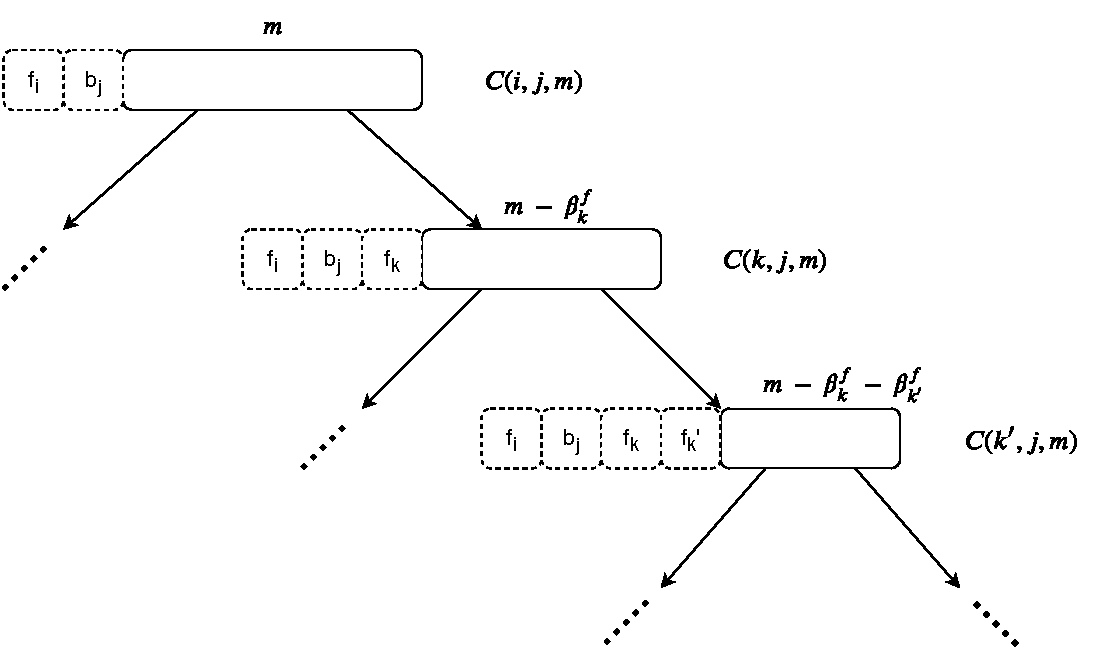
\includegraphics[width=0.83\linewidth]{b_j_placement_problem.pdf}
    \caption{The unrolling of two recursive calls into the right subproblems of \(C(i,\,j,\,m)\).}
    \label{fig:3-b-j-placement-problem}
\end{figure}

As per the definition of \(C(\cdot)\), we start with \(f_i\) and \(b_j\) already allocated in memory, and \(m\) memory left to work with to solve the problem.
We pick some checkpoint \(f_k\) and recurse on the right.
At the level of the subcall, \(f_k\) is defined as `already' in memory, separate from the \(m-\beta^f_k\) we have left to work with.
Once again, we pick some \(f_{k^\prime}\) and recurse on the right.
Now, \(f_{k^\prime}\) is already in memory, and we have \(m - \beta^f_k - \beta^f_{k^\prime}\) to work with.

As we recurse further right, shown in Figure \ref{fig:3-b-j-placement-problem-right}, this memory will get used up as we place more checkpoints, until eventually we place \(f_{j-1}\), at which point we can start the backwards pass.
We compute \(b_{j-1}\) from \(f_j\) and \(b_j\).
As shown in our analysis in Section \ref{sec:2-4-2-peak-mem-training}, we can now free \(f_{j-1}\) and \(b_j\).
As we proceed backwards freeing memory, eventually our subcall \(C(k^{\prime},\,j,\,m - \beta^f_k - \beta^f_{k^\prime})\) finishes with only the computed \(b_{k^\prime}\) sitting in the \(m - \beta^f_k - \beta^f_{k^\prime}\) memory.

However, notice that \(b_j\) was considered already allocated in memory elsewhere, separate to our workspace of size \(m - \beta^f_k - \beta^f_{k^\prime}\);
as we proceeded backwards, we had no control over whether \(b_j\) was freed so could not reclaim its memory and reuse it.
The problem is that a much further up supercall had fixed the allocation of \(b_j\), and only when it returns is \(b_j\) freed.
This is caused by defining \(C(\cdot)\) to say that \(b_j\) is already allocated outside of the \(m\) memory remaining, fixing its placement `early' in the supercall, and so it is not until the supercall returns that eventually it will be freed.

\begin{figure}[t]
    \centering
    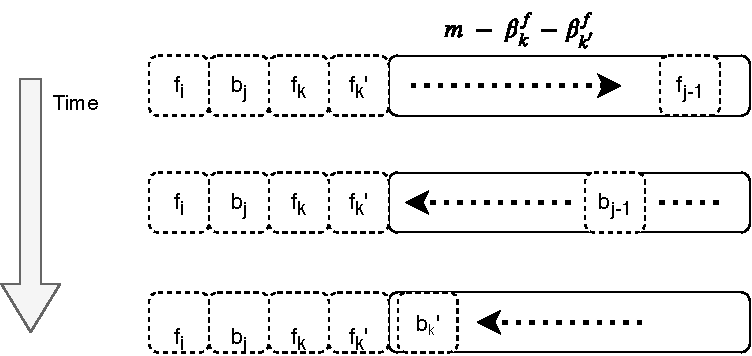
\includegraphics[width=0.6\linewidth]{b_j_placement_problem_recurse_further_right.pdf}
    \caption{Moving `right' until we finally reach \(f_{j-1}\), at which point we can move left, freeing tensors until only the ouput \(b_{k^\prime}\) remains.}
    \label{fig:3-b-j-placement-problem-right}
\end{figure}
Instead, we want to delegate responsibility of placing and freeing \(b_j\) down the subcalls, until eventually a subcall performs the backward step and can free it, reclaiming the memory.
Otherwise, when we start with \(C(0,\, N+1,\, m)\), the targets \(b_{N+1}\) will be kept allocated until the entire call has finished and we have gone all the way left to \(b_0\), rather than being the first backward at the end to get freed.
Each time we recurse on the left, the \(b_j\) for that call will also not be finished until we have proceeded all the way left to the \(b_i\) for that call.
Clearly, this definition of \(C(\cdot)\) has totally broken our memory analysis.
\begin{figure}[h]
    \centering
    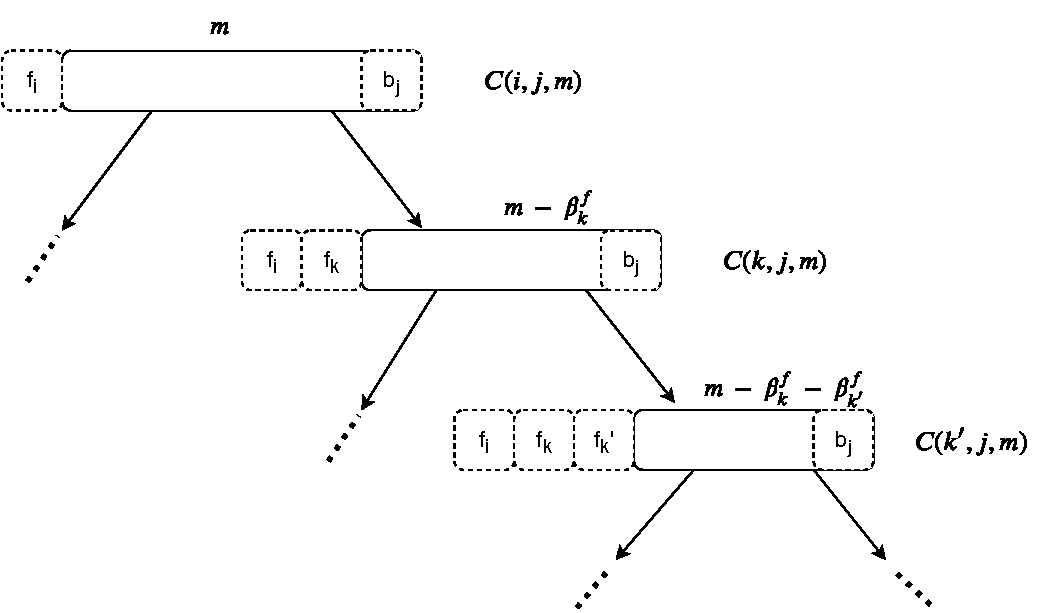
\includegraphics[width=0.77\linewidth]{b_j_placement_new.pdf}
    \caption{How \(b_j\) is now placed within \(m\), so the subcalls take ownership of placing it.}
    \label{fig:3-b-j-placement-new}
\end{figure}

Therefore, we redefine \(C(i,\,j,\,m)\) to mean that \(f_i\) is computed and already in memory, and \(b_j\) is computed, \textit{but we are responsible for placing \(b_j\) within our \(m\) memory and freeing it}.
This way, as we recurse down the subcalls, say to the right, we pass `ownership' of \(b_j\) to that subcall, which will place \(b_j\) within its own \(m-\beta^f_k\) memory and then free it as soon as possible.
This is visualised in Figure \ref{fig:3-b-j-placement-new}.

Now, as we keep recursing further right placing checkpoints, when we eventually reach \(f_{j-1}\), the subcall we are in can compute the backward step for \(b_{j-1}\) and free \(b_j\).
As the backward pass proceeds left, the backwards will now actually be freed, until we have gone back up to the \(C(k^\prime,\, j,\, m-\beta^f_k -\beta^f_{k^\prime})\) call and \(b_{k^\prime}\) is the only tensor left.
This is shown in Figure \ref{fig:3-b-j-placement-new-right}.
\begin{figure}[h]
    \centering
    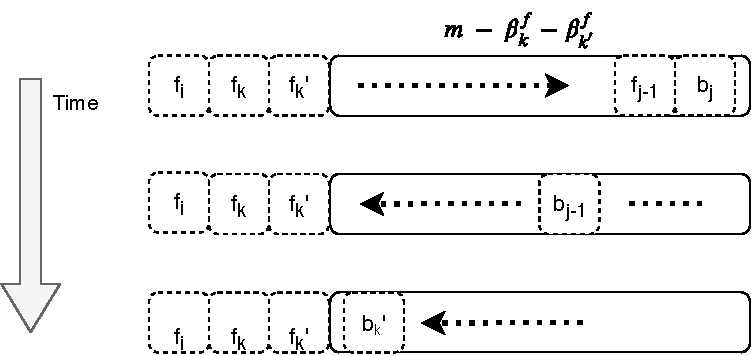
\includegraphics[width=0.6\linewidth]{b_j_placement_new_recurse_right.pdf}
    \caption{Demonstrating how the backwards will now actually be freed during the backwards pass}
    \label{fig:3-b-j-placement-new-right}
\end{figure}

This new definition of \(C(\cdot)\) of course affects our analysis of peak memory for \(Q(i,\,j,\,k,\,m)\) in Equation \ref{eqn:3-b-k-1}.
We must take into account the fact the \(b_j\) is using part of the \(m\) memory.
Thus, the first stage where we compute the forwards to \(f_k\) must be done within \(m-\beta^b_j\) memory.
Then, we recurse on the right with the same \(m-\beta^f_k\) memory as before, but now the definition of the subcall is that it must also place \(b_j\) within that memory.
By the time the subcall has finished, \(b_j\) will be long gone and \(b_k\) will be all that remains in its \(m-\beta^f_k\) memory.
We then recurse on the left with the same \(m\) memory as before;
the left subcall is now responsible for placing \(b_k\) within that \(m\) memory (and then freeing it), rather than saying \(b_k\) is in some separate memory to \(m\) whilst the left subcall proceeds.
\begin{figure}[h]
    \centering
    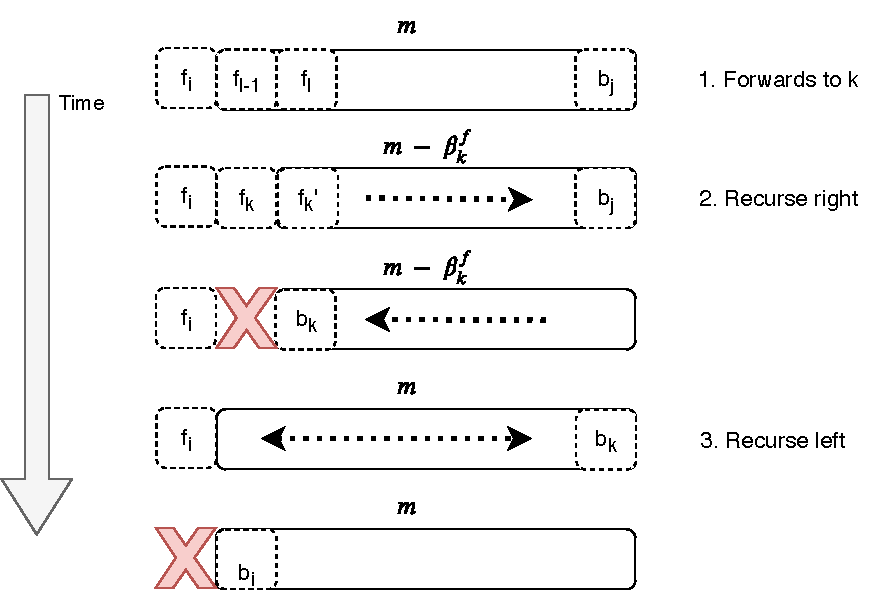
\includegraphics[width=0.7\linewidth]{new_Q_peak_mem.pdf}
    \caption{How peak memory occurs across the three stages of \(Q(\cdot)\).}
    \label{fig:3-new-Q-peak-mem}
\end{figure}

The peak memory across the three stages is visualised Figure \ref{fig:3-new-Q-peak-mem}.
Specifically, we update the peak memory of \(Q(i,\,j,\,k,\,m)\) as established in Equation \ref{eqn:3-b-k-1} to the following:
\begin{align} \label{eqn:3-b-k-2}
    \begin{aligned}[t] % so only one label for whole thing
        &\max(\\[0.5em]
        &\qquad\begin{aligned}[t]
            &\beta^b_j \,+\, \beta^f_{i+1}, \\[0.5em]
            &\beta^b_j \,+\, \max_{i+1 \,<\, l \,\leq\, k}\; \beta^f_{l-1} + \beta^f_l, \\[0.5em]
            &\beta^f_k \,+\, B(k,\, j,\, m\,-\,\beta^f_k), \\[0.5em]
            &B(i,\,k,\,m)
        \end{aligned} \\[0.5em]
        &)
\end{aligned}
\end{align}
As before, we will have to check each of these stages for failure before evaluating \(Q(\cdot)\).

%%%%%%%%%%%%%%%%%%%%%%%%%%%%%%%%%%%%%%%%%%%%%%%%%%%%%%%%%%%%%%%%%%%%%%%%%%%%%%%%
\subsection{The New Algorithm So Far}
In the above sections, I have accounted for per-layer costs; how to traverse the subproblem space; introduced \(B(\cdot)\); accounted for failure; and changed how the problem is modelled so the backwards actually get freed during the backward pass.

Let us take a breather from analysing the naunces of the problem, and instead consolidate the above changes into the new algorithm \textit{thus far}, shown in Algorithm \ref{alg:3-policy-solver-intermediate}.

There are a still a few minor details to note. First, whereas Gruslys et al. defined \(y = D(i,\, j,\, m)\) as the \textit{offset} to the next layer to checkpoint; I use \(k = D(i,\,j,\,m)\) as the \textit{index} of the forward tensor.

Second, according to our definition of \(C(i,\,j,\,m)\), the \(m\) memory budget does not include \(f_i\) but does include \(b_j\).
This means the largest subproblem on \((0,\,N+1)\) must be solved within \(M-\beta^f_0\) memory, not \(M\), as there must be enough space remaining in the original \(M\) to store \(f_0\) and separately compute \(C(0,\,N+1,\,m-\beta^f_0)\).

Also, \(\alpha^f_{N+1}\) and \(\beta^f_{N+1}\) are not actually defined tensors, but since \(\alpha^b_{N+1}\) and \(\beta^b_{N+1}\) are defined, I make the second dimension of their arrays \(N+2\).

Lastly, as arrays start at 0, but memory starts at 1, we will index \(B,\, C,\, D\) with \(m-1\) when referring to \(m\) memory.

\begin{algorithm}[htbp]
    \DontPrintSemicolon
    \SetKwData{PeakFs}{peak\textsubscript{F}}
    \SetKwData{Failed}{failed}
    \SetKwData{PeakR}{peak\textsubscript{R}}
    \SetKwData{PeakL}{peak\textsubscript{L}}
    \SetKwData{Peak}{peak}
    \SetKw{Continue}{continue}

    \KwIn{\(N\) the sequence length}
    \KwIn{\(M\) the memory budget}
    \KwIn{\(\alpha\) a \(2\times(N+2)\) \texttt{float} array of the per-operator compute costs}
    \KwIn{\(\beta\) a \(2\times(N+2)\) \texttt{int} array of the per-operator memory costs}
    \BlankLine
    
    \(M \;\leftarrow\; M \,-\, \beta^f_0\)\;
    \BlankLine

    Let \(B\), \(C\), \(D\) be 3D arrays of size \((N+1)\times(N+1)\times M\)\;
    \BlankLine

    Base cases will go here.\;
    \BlankLine

    \# Traverse the subproblems bottom-up.\;
    \For{\(m \;=\; 2\) \KwTo \(M\)}{
        \For{\(i \;=\; N\) \KwTo \(0\)}{
            \# Base case has already handled \((i,\,i+1)\), so start at \(i+2\).\;
            \For{\(j \;=\; i+2\) \KwTo \(N+1\)}{
                \(C_{min} \;\leftarrow\; \infty\)\;
                \Failed \(\;\leftarrow\; \top\)\;
                \For{\(k \;=\; i\,+\,1\) \KwTo \(j\,-\,1\)}{
                    \# Pre-check the stages of this strategy for failure.\;
                    \BlankLine

                    \# 1: Forwards to \(f_k\) in-place whilst holding \(b_j\).\;
                    \PeakFs \(\leftarrow\; \beta^b_j \;+\; \max(f_{i+1},\, \max_{i \,<\, l \,<\, k}\, \beta^f_l + \beta^f_{l+1})\)\;
                    \BlankLine

                    \If{\PeakFs \(>\, m\)}{
                        \Continue\;
                    }
                    \BlankLine

                    \# 2, 3: Right and left subproblems \;
                    \BlankLine

                    \If{\(m \,-\, \beta^f_k \,<\, m\)}{
                        \Continue\;
                    }
                    \BlankLine

                    \PeakR \(\;\leftarrow\; B[k][j][m-\beta^f_k-1]\)\;
                    \PeakL \(\;\leftarrow\; B[i][j][m-1]\)\;
                    \BlankLine

                    \If{\PeakR or \PeakL failed}{
                        \Continue\;
                    }
                    \BlankLine

                    \Peak \(\;\leftarrow\; \max( \)\PeakFs\(,\, \beta^f_k + \) \PeakR\(,\,\)\PeakL\( ) \)\;
                    \BlankLine

                    \If{\Peak\(\;>\; m\)}{
                        \Continue\;
                    }
                    \BlankLine

                    \# Success, a strategy works!\;
                    \Failed\(\;\leftarrow\; \bot\)\;
                    \BlankLine

                    \(c \;\leftarrow\; \sum_{l\;=\;i\,+\,1}^k \alpha^f_l \,+\, C[k][j][m-\beta^f_k-1] \,+\, C[i][k][m-1]\)\;
                    \BlankLine

                    \If{\(c \,<\, C_{min}\)}{
                        \(C_{min} \;\leftarrow\; c\)\;
                        \(B[i][j][m-1] \;\leftarrow\;\) \Peak\;
                        \(C[i][j][m-1] \;\leftarrow\; c\)\;
                        \(D[i][j][m-1] \;\leftarrow\; k\)\;
                    }
                }
                \If{failed}{
                    \(B[i][j][m-1] \;\leftarrow\;\) \textit{failure}
                }
            }
        }
    }
    \Return{\((C,\, D)\)}
    
    \caption{The new policy solver thus far, incorporating the changes from the above sections.}
    \label{alg:3-policy-solver-intermediate}
\end{algorithm}

%%%%%%%%%%%%%%%%%%%%%%%%%%%%%%%%%%%%%%%%%%%%%%%%%%%%%%%%%%%%%%%%%%%%%%%%%%%%%%%%
\subsection{More Memoisation of Costs}
% Notice we have done memoisation in the algo we are yet to discuss.
Now that we have the algorithm concretely written down, we can see further opportunity for memoisation.

First, as we go over the \(k\) loop, we need the cost of computing \(f_{i+1}\rightarrow f_k\).
Obviously, we can accumulate this over the loop, rather than summing from \(f_{i+1}\) each time.

We could memoise this fully over all possible subsequences, so when we move \(j\) right we already have the costs to \(j-1\), and when we move \(i\) left, we already have the costs from \(i+1\).
However, I do not think the extra effort is worth it.
The extra code to memoise over just the \(k\) loop is so little compared to the entire loop body that it hardly adds any cost, so further savings from full memoisation will not have much effect.

Likewise, across the \(k\) loop, we can memoise the peak memory of computing the forwards to \(f_k\); and likewise, I do not bother with `fully' memoising this.

%%%%%%%%%%%%%%%%%%%%%%%%%%%%%%%%%%%%%%%%%%%%%%%%%%%%%%%%%%%%%%%%%%%%%%%%%%%%%%%%
\subsection{Failure Propagation and Short-Circuiting}
In this section, I consider how failure propagates `up' through the search space.
If some \(i,\,j,\,m\) fails - as in even when using the constant memory strategy we cannot run the subsequence - then we definitely cannot do any sequence of which this is a subsequence.
That is, all \(i^\prime,\, j^\prime\) where \(i^\prime \,\leq\, i\) and \(j^\prime \,\geq\, j\) must fail too.

We can propagate this failure right through \(j\) easily, as it is the inner loop.
When we encounter the failed subsequence, we short-circuit and set all the \(i,\, j^\prime\) to failure, then break from the \(j\) loop.

Propagating left through \(i\) is more complex, as it is the outer loop.
If the failure occurred on \((i_\mathrm{F},\, j_\mathrm{F})\) We need to remove from the \((i,\,j)\) space iterated over by the loops all \((i^\prime,\, j_{\mathrm{F}})\) for \(i^\prime \,\leq\, i_\mathrm{F}\).
To clarify, I do not mean storing the \(j_\mathrm{F}\) at which we failed, then for each \(i^\prime \,\leq\, i\) we iterate to, doing the \(j\)s up to \(j_\mathrm{F}\), setting the rest to failure, and breaking from the loop.
I mean actually removing those elements from the search space altogether, so we never iterate to them, like we elide the \(j\) by breaking out of the the \(j\) loop.

I am sure any solution would greatly increase the code complexity and so even make it slower.
I do not even bother with the stated approach of storing \(j_\mathrm{F}\) and immediately short-circuiting when we hit it, as the algorithm will only have to run that one extra iteration for \(j_\mathrm{F}\) before realising failure and setting all \(j^\prime \,\geq\, j_{F}\) to failure.

%%%%%%%%%%%%%%%%%%%%%%%%%%%%%%%%%%%%%%%%%%%%%%%%%%%%%%%%%%%%%%%%%%%%%%%%%%%%%%%%
\subsection{Base Cases}
Finally, we consider the base cases of the algorithm.
Previously, in Algorithm \ref{alg:2-policy-solver}, these were when the sequence length \(t\) was 1;
when \(m\) was 1 so we employed the constant space strategy;
and when \(m \,\geq\, t\), so we employed the no recomputation strategy.

\subsubsection*{Unit Sequence Length}
We shall first address the unit sequence length case.
It corresponds to \(j \,=\, i+1\).
For the problem \(C(i,\,i+1,\,m)\), we are given \(f_i\) and \(b_{i+1}\), and simply need to run the backward operator to get \(b_i\).
Thus, the computational cost is \(C(i,\,i+1,\,m) \;=\; \alpha^b_i\).
Recall the definition of the subproblem means it is responsible for placing \(b_{i+1}\) within its memory, as well as of course \(b_{i}\).
This makes the peak memory cost \(B(i,\,i+1,\,m) \;=\; \beta^b_i \,+\, \beta^b_{i+1}\).
Also, we need to check for failure (that this memory cost is less than \(m\)) before actually setting \(C(\cdot)\) and \(B(\cdot)\).
If failure did occur, then, like explained above, we set all \((i, j^\prime)\) where \(j^\prime \,\geq\, i+1\) to failure, then skip over the rest of the \(j\) loop.
Finally, we do not need to explcitly set the policy \(D(\cdot)\) as the executor function will have a base case for \(j \,=\, i+1\) that performs the backward step.

Given that we have already set up the loops to traverse \textit{all} subproblems bottom-up, we do not need a separate loop beforehand for initialising \(C(\cdot)\) with this base case, like in the original Algorithm \ref{alg:2-policy-solver} for RNNs.
In fact, looking at our new Algorithm \ref{alg:3-policy-solver-intermediate}, we can see that, before the \(j\) loop starts, initialised to \(j\,=\,i+2\), we can handle the \(j\,=\,i+1\) base case first.

\subsubsection*{The ``No Recomputation Strategy''}
When there is enough memory, we do not need to trade-off any compute for memory.
Recall from Equation \ref{eqn:2-nn-peak-mem} the peak memory of running backpropagation on a sequence:
\begin{equation*}
    \max_{0 \leq i \leq N}\; \sum_{l\;=\;0}^i \beta^f_l + \beta^b_{i+1} + \beta^b_i
\end{equation*}
Figure \ref{fig:3-base-case-peak-mem} visualises some possibilities of what this looks like.

\begin{figure}[h]
    \centering
    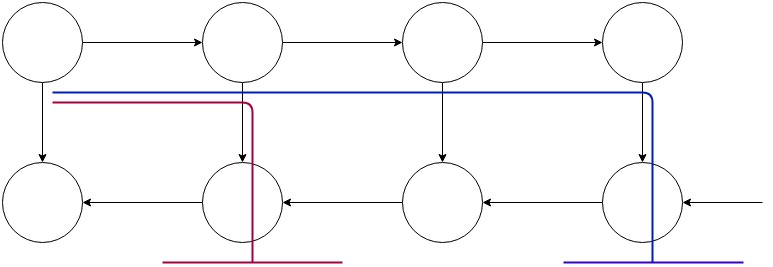
\includegraphics[width=0.7\linewidth]{no_recompute_peak_mem_vis.jpg}
    \caption{Two possibilities for when peak memory occurs. The blue line indicates peak memory occurs at the beginning of the backward pass. The red line indicates when we are computing the backward of the second layer.}
    \label{fig:3-base-case-peak-mem}
\end{figure}

The base case would be triggered for any subsequence we encounter where this expression is within \(m\).
That would be quite hard to memoise over and efficiently detect.
However, I have carefully crafted the \(j\,=\,i+1\) base case and the recursive case \(Q(\cdot)\) to have already accounted for this base case themselves.
The following outlines a proof of this.

First, consider a sequence of size one.
The \(j\,=\,i+1\) base case for this simply computes the single backward operator; it is vacuously true that no recomputation occurs.

Second, consider again the sequence of length greater than one in Figure \ref{fig:3-base-case-peak-mem}.
Let us say that its peak memory with no recomputation, represented by either of the coloured lines, is within the memory budget \(m\).
To find the optimal \(C(i,\,j,\,m)\), the algorithm will consider \(Q(i,\,j,\,k,\,m)\), for all \(i \,<\, k \,<\, j\).
That is, we break the problem down into the left subproblem \((i,\,k,\,m)\) and the right subproblem \((k,j,m-\beta^f_k)\).
For the optimal strategy of recomputing nothing to arise, we need the algorithm to choose to checkpoint the first forward, \(k\,=\,i+1\), and for the right subproblem to also checkpoint the first forward, and so on to \(f_{j-1}\); meaning everything was checkpointed and nothing was recomputed.
The left subproblem for each of these is the unit length base case so it is vacuously true that they involve no recomputation.

Consider the \(k\,=\,i+1\) case, where the right subproblem becomes \((i+1,\,j,\,m-\beta^f_{i+1})\).
Let \(c\) be the optimal computational cost when choosing \(k\,=\,i+1\).
By induction, let us say the optimal solution to this subproblem has correctly been found to be the no recomputation case.
Note it does not matter which backward step, shown as the coloured lines in Figure \ref{fig:3-base-case-peak-mem}, actually incurred the peak memory,
as either way, it is less than the memory budget by the definition of the problem, and has no bearing on whether we can say by induction that the right subproblem will have involved no recomputation.

So, in the \(k\,=\,i+1\) case, the cost \(c\) becomes the cost to compute \(f_i\rightarrow f_{i+1}\), plus the cost of the right subproblem, which involved no recomputation, plus the cost of the left subproblem, which will be over a single layer and so involves no recomputation.
Thus, choosing this strategy involves no recomputation, so it must be the optimal strategy that is picked by the algorithm, as it is impossible to beat the computational cost of doing no recomputation.

To show this, consider any other \(k^\prime\) with optimal cost \(c^\prime\).
Say its right and left subproblem involve no recomputation;
we get the same optimal cost \(c^\prime\,=\,c\) and so, regardless of whether the algorithm chooses \(k\) or \(k^\prime\), it will have found the optimal cost.
On the other hand, if either subproblem involved recomputation, then the cost cannot possibly be better than \(c\), so we choose \(k\) and get the no recomputation strategy.

Thus, we have (loosely) shown by induction that the algorithm already takes care of the ``no recomputation'' base case itself, so no further work is required to encode it in.

\subsubsection{The ``Recompute Everything'' Strategy}
Let us recap how this strategy works.
To perform backpropagation on the sequence \((i,\,j)\), we start with \(f_i\) and \(b_j\), then run the forwards in-place to \(f_{j-1}\).
The peak memory so far is the max of the forwards pair-wise across the layers we just ran, whilst holding \(b_j\) in memory.
Then, we compute \(f_{j-1}, b_j \,\rightarrow\, b_{j-1}\).
The peak memory for the entire first step then, is the max of the peak memory of each invididual forward step, whilst holding the upstream backward, and the backward step.
Next, we start again at \(f_i\), run the forwards in-place to \(f_{j-2}\) whilst holding \(b_{j-1}\), and compute \(f_{j-2}, b_{j-1} \,\rightarrow\, b_{j-2}\).
We repeat this until we have computed all the backward steps to \(b_i\).

Thus, the peak memory becomes the max of all the individual backward steps and, for each of those steps, the max of the forward steps to that layer whilst holding the upstream backward.
It is essentially the size of the single largest step required to perform backpropagation on the sequence.
The precise definition given below makes this more clear.
As explained in the previous sections, we will exclude the memory of \(f_i\) but include \(b_j\).
This cost is \(\Theta(1)\) with respect to the number of layers.
\begin{align*}
\begin{aligned}[t] % so only one label for whole thing
    &\max(\\[0.25em]
    &\qquad\begin{aligned}[t]
        &\max_{i\,<\, j^\prime \,<\, j}\; \beta^b_{j^\prime+1} \,+\, \max_{i+1\,<\, l \,<\,j^\prime}\; \beta^f_{l-1} \,+\, \beta^f_l, \\[0.5em]
        &\max_{i\,\leq\, l \,<\, j}\; \beta^f_l \,+\, \beta^b_{l+1} \,+\, \beta^b_l, \\[0.5em]
    \end{aligned} \\[0.25em]
     &)
\end{aligned}
\end{align*}

The computational cost of this strategy is \(\Theta(N^2)\); first we do \(j-i\) forward steps, then \(j-i-1\) steps, down to a single step.
In total, the first forward will be computed \(j-i\) times, the second \(j-i-1\) times, and so on, with the last forward only being computed once on the first step.
We do each of the \(j-i\) backward steps once.
This gives the precise computational below.
In accordance to the definition of \(C(\cdot)\), we do not count the cost of computing \(f_i\) or \(b_j\).
\begin{equation*}
    \sum_{l\;=\;1}^{j\,-\,i\,-\,1} (j\,-\,i\,-\,l) \cdot \alpha^f_{i+l} \;+\; \sum_{l\;=\;i}^{j-1}\alpha^b_l
\end{equation*}
% f_i to b_j
% f_i+1 to f_j-1
% b_i to b_j-1

% f_i+1: j-i-1
% f_i+2: j-i-2
% ...
% f_i+(j-i-1): j-i-(j-i-1)

explain how to memoise....
% The quadratic case has peak mem of whichever specific f_i->f_k, f_k,b_k+1->b_k, has the highest peak mem. If the peak mem of quadratic > m, we fail
% How to calculate this peak mem efficiently? That is, clearly in the already done subproblems we have already evaulated the peak mem of a lot of the computations that occur in the quadratic case.
% As we iterate from some j-1 to j, most of the quadratic computation is the same, so we should be able to memoise this result to efficiently calculate peak mem for i,j.
% we update a max_per_layer = max(max_per_layer, f_i to f_j, b_j)
%
% Theoretically, we could memoise this properly over all subsequences, not just across the j's for each i. That is, as we go left with i, we could also memoise this peak cost.
% However, this becomes complicated due to the fact that i-1,j modelled i-1 as not in the m memory, whereas i,j models i-1 as in memory. This means we cannot `induct' over the i-1,j possiblity because, if it was the case that i-1,j causes the peak memory, and not some k, k>i-1, then we cannot directly compared the memoised value with the i-1,j case.
% Furthermore, I believe the cost savings of this memoisation would be minimal, considering the memoisation across the j loop only adds a tiny bit of code to an already quite large loop body.
% the extra work involved in working around the above problem may even cause it to be slower!

% Anyway, as for each i, we work out peak per layer cost for quadratic case by memoising over j, the quadratic case becomes a part of the main loop, not some base case we set beforehand.
% So, if the recursive case failed for all k, we use our memoised value to see if quadratic can be done, else we fail for this i,j.

% also, the other j=i+1 base case can just be a part of the main loop too, as we iterate over all subproblems in order. At the top of the i loop, we consider i,i+1 before moving into the j loop for j=i+2...
% Thus, no separate base case loop like in the deepmind algo

% Finally we are done! Full algorithm:
